\begin{comment}

\section{Paradigmatic Models}
	\subsection[Classical]{Classical Model}

\begin{frame}
	\frametitle{Classical Ising Model}
	
	2D Classical Ising Hamiltonian with size $L$x$L$ and with PBC:
	\begin{columns}
		\begin{column}{0.5\textwidth}
		
		
\begin{figure}[!h]
		\centering
		\begin{tikzpicture}
			\begin{axis} [width=8cm,height=3.2cm,xmax=1, axis lines=middle, 
			enlargelimits,
			xtick={0.5},ytick={0.},xticklabels={$T_c$},yticklabels={$ $}, 
			xlabel=$T$,ylabel=$w$]
				\draw [dashed, line width=0.5pt,gray] (50,-60) -- (50,60);
				\node[text=blue] at (30,7) {\scriptsize{$M>0$}};
				\node[text=blue] at (30,-8) {\scriptsize{$M<0$}};
				\node[text=red] at (70,7) {\scriptsize{$M=0$}};
				\node[text=red] at (70,-8) {\scriptsize{$M=0$}};
				\node[text=red] at (70,-8) {\scriptsize{$M=0$}};
				\addplot [domain=0:0.5, samples=10,smooth,thick,black] {0};
				\filldraw [red] (49,-0.7) rectangle ++(3pt,3pt); %circle (3pt)
			\end{axis}
		\end{tikzpicture}
	\end{figure}			
	
		\end{column}
		\begin{column}{0.5\textwidth}
		
	\begin{align} % \vec
		H_{\rm cl} = - J\,\sum_{\braket{i,\,\,j}}  &
		S_i \cdot  S_j -  w \cdot \sum _i  S_i  \,\,,\\
		Z = \sum _{\{S_i\}} &\, e^{-H/T}  \,\,;
	\end{align}			
	
		\end{column}
	\end{columns}
	
	\bigskip
	
	\alert{\bf Continuous Transition point:} 
	at $w = 0$ and $T_c =  \frac{2}{\ln(1+\sqrt{2})}\,\,(J=1\,\,{\rm fixed})$\\
	$ $\\
	\alert{RG dimensions}:	
	\begin{align}
		w \longrightarrow y_w = 15/8 \qquad 
		T \longrightarrow y_t =  1	\qquad
		{\rm Metropolis \,\,time}\,\,t \longrightarrow z = 2.1667(5) \,\,.\notag
	\end{align}
\end{frame}


	\subsection[Quantum]{Quantum Models}


\begin{frame}
	\frametitle{Quantum Ising Model}
	
	1D Quantum Ising Hamiltonian for a chain of size $L\,$ and PBC 
	($\hat \sigma_{L+1}^{(k)} = \hat \sigma_1^{(k)}$):
	\begin{align}
		\hat H_{\rm Is} = -\sum_{x=1}^{L} \hat \sigma^{(1)}_x \hat
  		\sigma^{(1)}_{x+1} - g\, \sum_{x=1}^L \hat \sigma^{(3)}_x 
  		- w \sum_{x=1}^L \hat \sigma_x^{(1)}\,\,;
	\end{align}
	$\sigma^{(k)} _x$ are the Pauli matrices on the $x^{\rm th}$ site in the
	$k$-axis direction.
	
	\bigskip
	\bigskip
	
	\alert{\bf Continuous Transition point:} 
	at $w = 0$ and $g_c = 1$\\
	\alert{RG dimensions}:	
	$ $\\
	\begin{align}
		w \longrightarrow y_w = 15/8 \quad 
		& r = g-g_c \longrightarrow y_r =  1	\quad
		{\rm  time}\,\,t \longrightarrow z = 1 \\
		&\hat \sigma _x^{(1)} \longrightarrow y_l = d + z - y_h = 1/8\,\,.\notag
	\end{align}
	
\end{frame}
\end{comment}

%\section{Kitaev model}
\begin{frame}
	\frametitle{Kitaev Model}
	Kitaev Hamiltonian mapped into a spin-$1/2$ XY chain, by a 
	Jordan-Wigner transformation (OBC):
	$\qquad \qquad\alert{\hat c \longrightarrow \hat\sigma}\,$
	\begin{align}
		\label{KitaevH}
		\hat H _K^{\rm (ABC)} =- \sum _{x=1}^{L}\biggr[ \bigl(
		 \hat c_x^\dagger \, \hat c_{x+1} + 
		 \hat c_{x+1}^\dagger \,\hat c_x \bigl) + 
		 \delta\,\bigl( \hat c_x \, \hat c_{x+1} + 
		\hat c_{x+1}^\dagger \, \hat c_x^\dagger \bigl)\biggr] - 
		\sum _{x=1}^L  \mu \, \hat c_x^\dagger \, \hat c_{x}  \,\,;
	\end{align}
	\begin{figure}[!h]
		\centering
		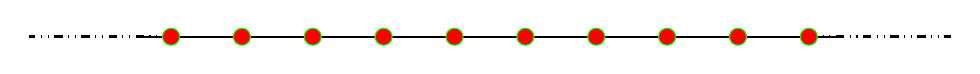
\begin{tikzpicture}[scale=0.9]
			\draw [-, line width=0.8pt, black] (-5.5,0.5) -- (4.5,0.5);

			\draw [dash dot dot, line width=1.2pt, black] (-5,0.5) -- (-7,0.5);
			\draw [dash dot dot, line width=1.2pt, black] (4,0.5) -- (6,0.5);

			\fill [red, draw=green] (-5,0.5) circle (0.12);
			\fill [red, draw=green] (-4,0.5) circle (0.12);
			\fill [red, draw=green] (-3,0.5) circle (0.12);
			\fill [red, draw=green] (-2,0.5) circle (0.12);
			\fill [red, draw=green] (-1,0.5) circle (0.12);
			\fill [red, draw=green] (4,0.5) circle (0.12);
			\fill [red, draw=green] (3,0.5) circle (0.12);
			\fill [red, draw=green] (2,0.5) circle (0.12);
			\fill [red, draw=green] (1,0.5) circle (0.12);
			\fill [red, draw=green] (0,0.5) circle (0.12);
			%\node (n) at (-4.5,0.85)  {$\bm{\hat c_1} $};
			%\node (n) at (4.5,0.95)  {$\bm{\hat c_L^\dagger} $};
		\end{tikzpicture}
	\end{figure}

	\alert{\bf Continuous Transition point:} 
	\begin{align}
		\mu _c = -2 \qquad {\rm and} \qquad \delta = 1 \,\,{\rm fixed} \,\,;\notag
	\end{align}
	\alert{RG dimensions}:	
	$ $\\
	\begin{align}
		w = \mu - \mu_c \longrightarrow y_w = 1 \qquad 
		\hat c_x \, ,\,\, \hat c_x^\dagger \longrightarrow y_c = 1/2 \qquad
		{\rm dynamic \,\, exp:\,\,} z =1
		\,\,.\notag
	\end{align}
	
\end{frame}
